\section{Navigazione della scena}
\label{sec:chapter_caso_uso_navigazione_scena}

L’utente che vuole fruire in ambiente web di una scena 3D realizzata in Three.js deve accedere al servizio di navigazione mediante l’ apposito URL. 
\\
Una volta effettuato l’accesso, l’utilizzatore deve caricare la scena creata precedentemente in Three.js tramite il pulsante IMPORT inserito nel menu in alto a destra.
\\
La scena verrà quindi mostrate su schermo mediante una visuale dall’alto in cui è permesso modificare il punto di vista tramite l’utilizzo del mouse, del trackpad o  del touch screen nel caso in cui venga utilizzato uno smartphone/tablet.
\\
\begin{figure}[htb]
 \centering
 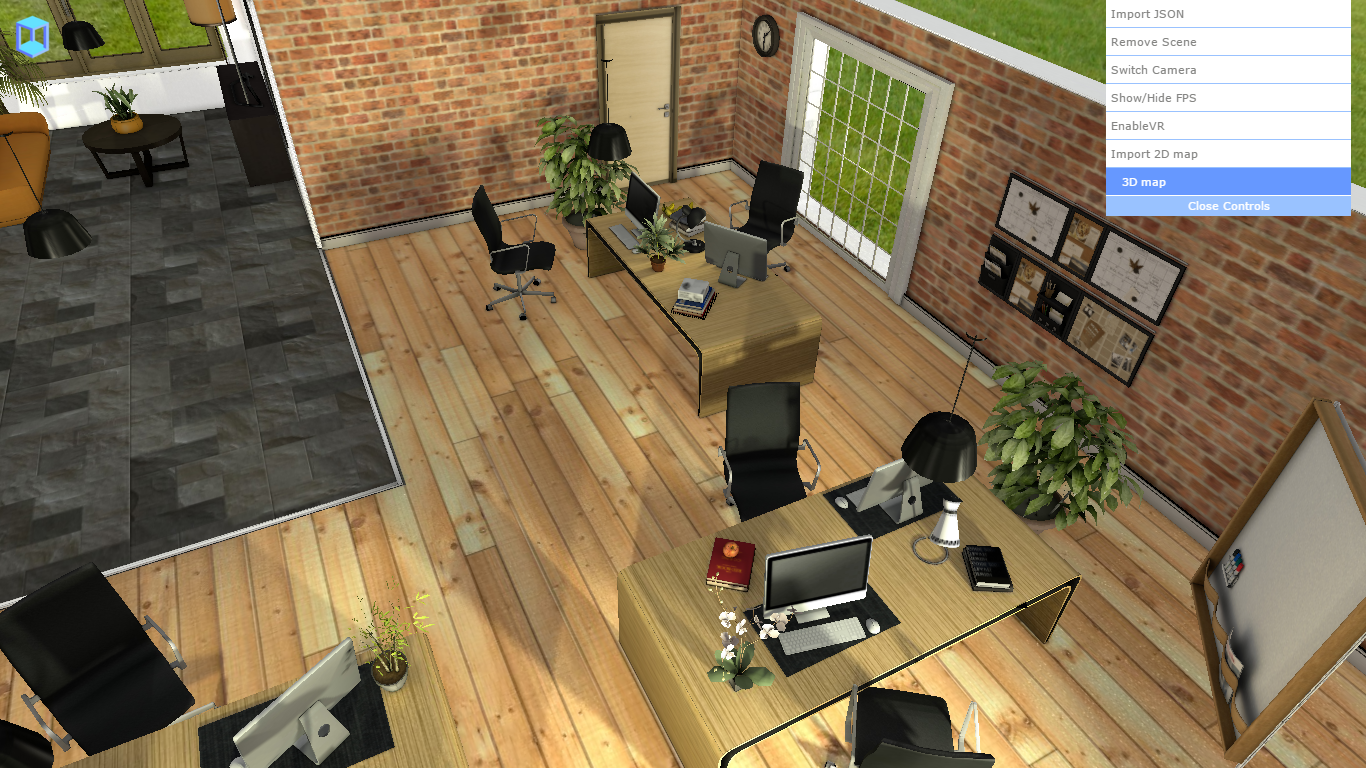
\includegraphics[width=1\linewidth]{images/chapter_caso_uso/vista_alto.png}\hfill
 \caption[Esempio di vista dall'alto]{Un esempio di vista dall'alto ottenuta con il navigatore}
 \label{fig:caso_uso_vista_alto}
\end{figure}

Una volta caricata la scena, l’utente può decidere se cambiare la modalità di osservazione passando da una vista dall’alto ad una in prima persona e viceversa, tramite l’utilizzo del pulsante \emph{SWITCH CAMERA}.
La vista in prima persona permette all’utente di navigare la scena simulando il comportamento  reale di una persona che visita realmente l’appartamento.
\\
Di default, quando l’utente utilizza questa modalità, verrà mostrata in alto a destra la mappa generata automaticamente della scena osservata  dall’alto in cui viene riportata tramite un indicatore la posizione dell’osservatore all’interno dell’ ambiente.
\\
L’utente utilizzando la voce \emph{3D map} nel menu può inoltre decidere se mostrare all’interno della mappa l’intera scena oppure solamente i muri ed i pavimenti dell’abitazione.
Inoltre all’interno della voce \emph{3D map} è possibile scegliere se disibilitare completamente la mappa durante la navigazione in prima persona.
\\
All’ utente infine viene anche data la possibilità di importare una mappa 2D creata ad hoc per la scena, descritta all’interno di un json appositamente creato.

IMMAGINE


Quando la navigazione in prima persona viene avviata da un pc fisso o portatile,  l’utente può visitare la scena mediante l’utilizzo combinato di tastiera e mouse.
Per muoversi all’interno della scena vengono utilizzati i pulsanti della tastiera \emph{W,A,S,D} che permettono il movimento rispettivamente in avanti, a sinistra, in basso, a destra.
\\ 
La pressione di due pulsanti adiacenti nella tastiera permette il movimento nelle quattro direzioni oblique. Lo spostamento del mouse permette invece l’osservazione della scena in direzioni differenti.
Il pulsante barra spaziatrice permette infine di simulare il salto dell’osservatore nella scena importata.
\\
Come descritto precedentemente, in alto a destra verrà mostrata, se inserita, la mappa creata automaticamente dall’editor oppure quella 2D creata ad hoc dall’utente.
In ogni momento durante la navigazione, l’utente può decidere di mettere in pausa la navigazione tramite la pressione del pulsante \emph{esc}.
\\
Durante la pausa è possibile utilizzare nuovamente il menu in alto a destra, che viene nascosto quando la visita in prima persona è attivata.

IMMAGINE


Se l’utente utilizza il navigatore da smartphone e possiede gli occhiali \emph{Google VR}  può sfruttare la modalità che permette la visione stereoscopia 3D della scena creata, attivabile tramite il pulsante \emph{EnableVR}.
\\
La scena passa quindi in modalità di navigazione in prima persona e viene navigata sfruttando l’oscilloscopio del telefono.
\\
\begin{figure}[htb]
 \centering
 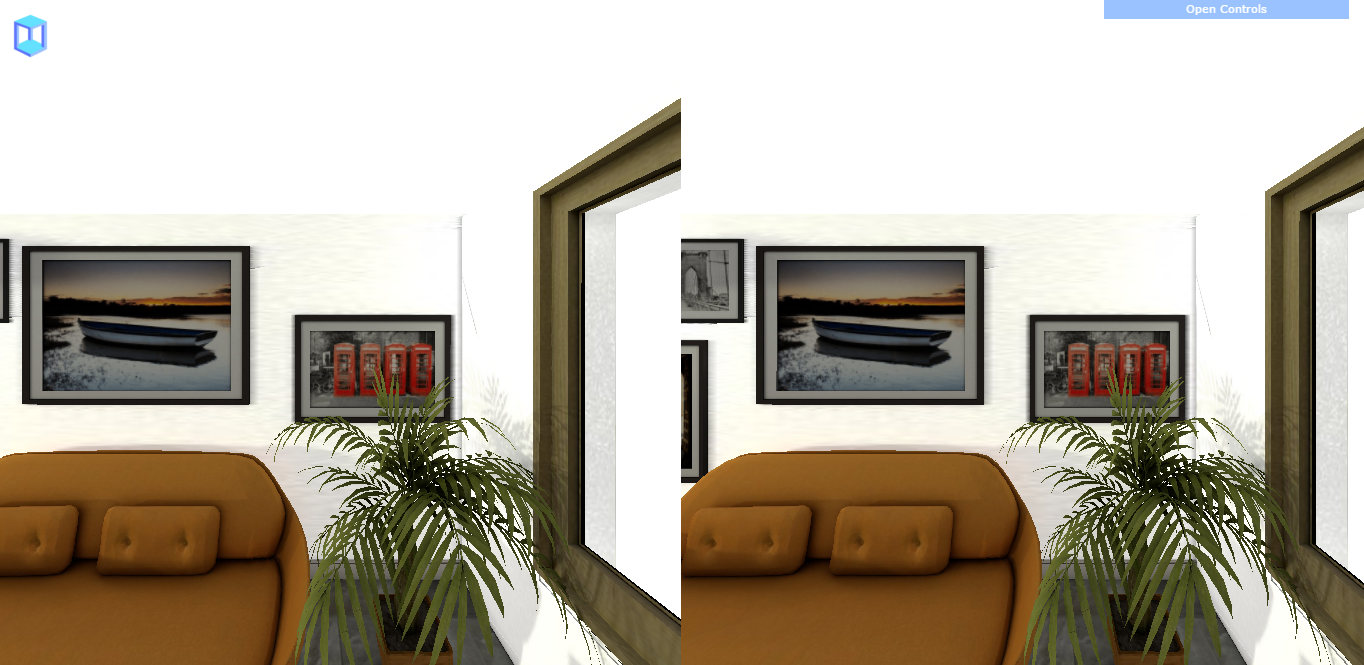
\includegraphics[width=1\linewidth]{images/chapter_caso_uso/google_vr.png}\hfill
 \caption[Esempio di visione stereoscopica 3D]{Un esempio di visione stereoscopica 3D}
 \label{fig:caso_uso_vista_alto}
\end{figure}

Il movimento avviene automaticamente in avanti secondo la direzione di osservazione, quest’ultima viene modificata mediante l’utilizzo dell’oscilloscopio del cellulare.


